\documentclass[
	%parspace, % Térköz bekezdések közé / Add vertical space between paragraphs
	%noindent, % Bekezdésének első sora ne legyen behúzva / No indentation of first lines in each paragraph
	%nohyp, % Szavak sorvégi elválasztásának tiltása / No hypenation of words
	twoside, % Kétoldalas nyomtatás / Double sided format
	final, % Teendők elrejtése / Set final to hide todos
]{elteikthesis}[2019/06/10]

% Dolgozat metaadatai
% Document's metadata
\title{Automatic Spine Vertebrae Segmentation from CT Images } % cím / title
\date{2021} % védés éve / year of defense

% Szerző metaadatai
% Author's metadata
\author{Kumundzhiev Maxim}
\degree{programtervező informatikus MSc}

% Témavezető(k) metaadatai
% Superivsor(s)' metadata
\supervisor{Szűcs Ádám István} % belső témavezető neve / internal supervisor's name
\affiliation{doctoral candidate} % belső témavezető beosztása / internal supervisor's affiliation
%\extsupervisor{Külső Kornél} % külső témavezető neve / external supervisor's name
%\extaffiliation{informatikai igazgató} % külső témavezető beosztása / external supervisor's affiliation

% Egyetem metaadatai
% University's metadata
\university{Eötvös Loránd Tudományegyetem} % egyetem neve / university's name
\faculty{Informatikai Kar} % kar neve / faculty's name
\department{Komputeralgebra Tanszék} % tanszék neve / department's name
\city{Budapest} % város / city
\logo{elte_cimer_szines} % logo

% Irodalomjegyzék hozzáadása
% Add bibliography file
\addbibresource{thesis.bib}

% A dolgozat
% The document
\begin{document}
	
% Nyelv kiválasztása
% Set document language
%\documentlang{magyar}
\documentlang{english}

% Teendők listája (final dokumentumban nincs)
% List of todos (not in the final document)
\listoftodos[\todolabel]

% Dokumentum beállítások
% Some document settings
% Lábjegyzet folytonos számozása fejezetek között
% Contiunous counting of footnotes among chapters
\counterwithout{footnote}{chapter}

% Tartalomjegyzék oldalszámozásának rejtése
% Hide page numbering of ToC
\newcounter{conpageno}
\let\oldtableofcontents\tableofcontents
\renewcommand{\tableofcontents}{
	\pagenumbering{gobble}
	\oldtableofcontents
	\cleardoublepage
	\setcounter{conpageno}{\value{page}}
	\pagenumbering{arabic}
	\setcounter{page}{\value{conpageno}}
}


% Címlap (kötelező)
% Title page (mandatory)
\maketitle
\topicdeclaration

% Tartalomjegyzék (kötelező)
% Table of contents (mandatory)
\tableofcontents
\cleardoublepage

% Tartalom
% Main content
Medical imaging consists of set of processes or techniques to create visual representations of the interior parts of the body such as organs or tissues for clinical purposes to monitor health, diagnose and treat diseases and injuries. Moreover, it also helps in creating database of anatomy and physiology.
A group of processes for creating visual representations of the interior parts of the body such as organs or tissues are called medical imaging. This technique is used for clinical purposes to monitor health, diagnose and treat diseases and injuries. Additionally, it also helps to generate a database of anatomy and physiology.

Owing to the advancements in the field today medical imaging has the ability to achieve information of human body for many useful clinical applications. Different types of medical imaging technology gives different information about the area of the body to be studied or medically treated.
There is a lot of progress in medical imaging today. Thereby this field enables reach information on the human body for many valuable clinical applications. Various types of medical imaging technology provide different information regarding the area of the body which needs to be studied or medically treated.
 
Organisations incorporating the medical imaging devices include freestanding radiology and pathology facilities as well as clinics and hospitals.
Freestanding radiology, pathology facilities, clinics, and hospitals are organizations where are medical imaging devices are used.

The use of medical imaging for diagnostic services is regarded as a significant confirmation of assessment and documentation of many diseases and ailments. High quality imaging improves medical decision making and can reduce unnecessary medical procedures.
Implementation of medical imaging in diagnostic services is considered to be an important validation of evaluation and documentation of many diseases and ailments. For improving medical decision-making and reducing pointless medical procedures high-quality imaging is used.

Earlier diagnosis included exploratory procedures to figure out issues of ageing person, children with chronic pain, detection of early diabetes and cancer. With the advent of medical imaging the vital information of health can be made available from time to time easily which can help diagnose illnesses like pneumonia, cancer, internal bleeding, brain injuries, and many more.

Earlier diagnosis contained exploratory procedures to find out issues of elderly people, children with chronic pain, detection of early cancer or diabetes. Illnesses like cancer, internal bleeding, brain injuries, pneumonia, and many more can be diagnosed much more easily with the advent of medical imaging because the vital information of health becomes more available.

Doctors perform medical imaging to determine the status of the organ and what treatments would be required for the recovery. The choice of imaging depends on the body being examined and the health concern of the patient. Therefore, patients are tested before if their body reacts affirmatively to the radiation used for medical imaging and making sure least possible amount of radiation is used for the process. Moreover, proper shielding is done to avoid other body parts from getting affected.

There are many different types of imaging, such as X-rays, CT (computed tomography) scans, MRI (magnetic resonance imaging) and ultrasound. Each imaging type uses a different technology to create an image. This increasing range of imaging types provides health professionals with many options for showing what is happening inside your body.

Medical imaging to capture the spine is a key tool used in clinical practice for diagnosis and treatment of patients suffering from spinal conditions. A common image modality used in clinics is Computed Tomography (CT), which provides a detailed view of the spinal anatomy. Once a scan of a patient is acquired the scan must be analyzed. 

One such analysis would be to locate and identify which vertebrae are visible within the scan. However, this is not a trivial task, is error-prone and can be time- consuming. First, as CT scans use X-rays the exposure to the patient is often limited by only scanning the part of the body which is of interest. This means that a limited number of vertebrae are captured in each scan. These scans, known as arbitrary Field-Of-View (FoV) scans, make the vertebrae harder to identify because a radiologist cannot simply count from the end of the column or because they miss important visual context. Second, the scans often include severe pathological cases which could mean that the spine is an abnormal shape or the scan could be post-op and contain metal implants causing imaging arti-facts. Third, many vertebrae have similar appearance and are hard to tell apart without contextual, anatomical information. 
An algorithm which could perform the task of vertebrae localization and identification could not only inform radiologists and speed up their workflow, it could also be used as prior information for subsequent algorithms, for example, a lesion or fracture detection algorithm. In addition, automation could be used to perform a survey over a large dataset of spines to record information about a population, a task which is difficult to do manually by human experts.
The same reasons that make this problem hard for radiologists also make it difficult for an algorithm. In 2012, Glocker et al. [4]. proposed a solution to the problem which regressed the centroid positions however the method made assumptions about the shape of the spine and thus did not work well on patho- logical cases. Later, in [5] this was improved upon from their previous solution by turning the problem from a regression into a dense classification problem. This was done by generating a dense labelling, which is a label given to each pixel in the scan, from the ground-truth centroid annotations. The dense labelling is then converted back to the sparse labelling of centroid positions at the end of the processing pipeline. This approach worked much better for pathological cases. Both approaches [4,5] used random forests but there has since been an emergence of convolutional neural networks (CNN) in medical image analysis [3,7,10] and better results have been achieved for the vertebrae localization task with deep learning [2]. Some use a U-net architecture, such as Yang et al [11], which is a popular architecture for image segmentation problems [9]. In 2018, Liao et al. [6] published a state-of-the-art solution which regresses the positions of the centroids using a CNN combined with a Recurrent Neural Network (RNN) to capture the ordering of the vertebrae and to incorporate long-range contex- tual information. Based on the literature, we decided to develop a new approach which should have the following features: 1) Use CNNs, 2) Capture the order- ing of the vertebrae to improve accuracy, 3) Use a Dense Labelling strategy and turn the problem into a classification task, 4) Capture short and long-range contextual information from the scan.

\cleardoublepage

\chapter{Related works}
\label{ch:rworks}


\cleardoublepage


\chapter{Computer vision basics}
\label{ch:computer_vision_basics}

\section{Prehistory} %There is no such thing as prehistory here, background or history rather
The continuous advancing until nowadays covers the birth of neural nets with the perceptron, the famous AI winter and neural nets restitution with back-propagation as well as research resurgence in 2003's once GPU was spread wide scale-wise. Many of the basics which we developed in between 1980s and 1990s are still handy and are the basic mathematical apparatus of complex neural network architectures. As a result, nowadays we can overwatch the situation of incredibly fast developing and establishing new state of the art models almost each week. 

The huge shift detached by increased computational power and what is more impactfully - increased amount of generated data by human day-wise. The biggest amount of data year-wise was produced by people for the last two years.

The occurrence of the graphics processing unit enhanced the computational processing speed in 10000 times in the span of the last 15 years. As for exponential rise in data, nowadays technology allows us to store and manage data more times efficient even rather it was few years ago. 


The conjunction of significant technologies and highly-frequently generated data almost in every human-wise field, allowed deep learning as the science field as well as for researches to invent and deliver more robust and scope-wise models.

Below it is presented a very short list of achievements and insights for 2020th in different Deep Learning fields:
\begin{itemize}
 % add citation: https://www.nytimes.com/2020/11/24/science/artificial-intelligence-ai-gpt3.html
  \item \emph{NLP}: It was delivered GPT-3 - This summer, an artificial intelligence lab in San Francisco called OpenAI unveiled a technology several months in the making. This new system, GPT-3, had spent those months learning the ins and outs of natural language by analyzing thousands of digital books, the length and breadth of Wikipedia, and nearly a trillion words posted to blogs, social media and the rest of the internet.
  % add citation: https://thinkml.ai/top-5-ai-achievements-of-2020/
  \item \emph{Healthcare and Drug Discovery}: AI-based advancements in healthcare are one of the most beneficial uses of AI to mankind as it comes with offering speedy treatment strategies. For instance, InSilico Medicine developed a new potential drug with researchers from the University of Toronto; that particular drug can prevent tissue scarring in forty-six days only. Furthermore, it requires ten years to develop potential medications with an average cost of \$2.6 billion, but AI promises to do the same task in less time and less budget.
  % add citation: https://thinkml.ai/top-5-ai-achievements-of-2020/
 \item \emph{COVID-19 Detection in Lungs by AI}: The scientists at the University of Central Florida conducted a study to use artificial intelligence in the detection of COVID-19 in the lungs. The present study is efficient enough to lessen the testing challenges as the system is as accurate as a specialist medical doctor. They trained AI algorithms to identify COVID-19 pneumonia with ninety percent accuracy via computer tomography (CT) scans. It has identified 84 percent positive and 93 percent negative cases at present.
 % add citation: https://thinkml.ai/top-5-ai-achievements-of-2020/
 \item \emph{Video Analysis and Computer Vision}: Advancement in artificial intelligence and deep learning made a video or image analysis more feasible with cheaper investment. Much medical equipment in the field of radiology has crossed human efficiency to diagnose certain diseases. These techniques are helping physicians in their daily patient-checkups by making them accurate and quick. Computer vision technologies are greatly influencing the manufacturing industry in offering automatic quality control and safety management techniques.
\end{itemize}


\section{Core Concepts}
Within core concepts it will be descried machine learning as field itself, feature engineering, feature learning, feature representation, logistic classifier, data managing, structure of naive neural network, linear model of neural network, loss functions, optimizers, multi layer perceptron, non-linearity, convolutional neural networks, transfer learning and fine tuning concepts within example MNIST. %IF NOT MNIST CHANGE      

\subsection{Machine Learning}
Today machine learning (ML) is one of the sub-fields of data science strived to build complex systems that may find patterns in labeled and unlabeled data sources by issuing analysis of data jointly application of various algorithms. The patterns quite frequently are latent for usual people and what makes ML more desired and useful for different applications.  Welly fitted  ML models may produce accurate predictions for upcoming unlabeld data.



Computers today work side by side with humans. Every time we use banking services, shop online, or communicate on social media, machine learning algorithms help make this interaction more convenient, efficient and secure. Machine learning and related technologies are evolving rapidly. Their capabilities today are just the tip of the iceberg.

First we take some data, train a model off that data, then use that model to make predictions on brand new data.  Training is analogous to how humans learn.  The model is exposed to new data, makes a prediction, and gets feedback about how accurate its prediction was.  It uses that feedback to correct errors inside the model.\footnote{In contrast, unsupervised learning eliminates the feedback portion and looks for unlabeled underlying structure.} This process is repeated step by step multiple times through the entire data set. 

The input data has $n$ observations and $m$ features.  Features are attributes about the input data.  For example, take a bank.  There are $n$ customers who have $m$ features such as \textit{does someone have a checking account?  How much money is in that account?}    

Machine learning models have the ability to predict either continuous values (\textit{How much will someone spend per month?}) or classify $k$ discrete values (\textit{will someone open a savings account?}).   These discrete values are referred to as \emph{classes}.  In the classification example, the output has $k = 2$ classes (\textit{yes} or \textit{no}). This paper will focus on classification.

\subsection{Feature Engineering}
\emph{Feature engineering} is the process of using domain knowledge of data to extract useful features or patterns to make machine learning easier.  For example, say you were training a model to predict if a photo was taken indoors or outside.  You know that the sky is blue and so the percentage of blue pixels might be a good indicator (feature).  By engineering that feature ahead of time, the model does not have to learn that the sky is in fact blue.  This reduces the number of classes the model needs to consider (percentage of blue pixels vs. sky is blue or green or white).  Examples of feature extractors for images are SIFT, HOG, RIFT.  
% * <darren@myhigherground.com> 2016-05-19T03:42:41.143Z:
%
% > This reduces the number of classes the model needs to consider.
%
% needs another sentance for clarification 
%
% ^ <nreis@ucdavis.edu> 2016-05-19T16:09:51.417Z.

While feature engineering is still a very important skill, it has its drawbacks.  It requires expert knowledge of the problem, it can be very problem specific, and it takes a lot of hand tuning - which is time consuming.  
\subsection{Feature Learning}
\emph{Feature learning} is the process in which the algorithm autonomously finds distinguishing patterns, extracts them, and then feeds them to the classification layer.  In other words, feature learning is feature engineering done automatically by algorithms.  In deep learning, convolutional neural networks [CovNet] form a hierarchy of abstraction that grow in complexity (blobs$\rightarrow$edges$\rightarrow$eyes, noses, ears $\rightarrow$ face), see Fig \ref{fig:FeatLearn}.  The final layer takes this generated feature and uses it for classification.\cite{NvidiaConcepts} 

\begin{figure}[!h]
 \begin{center}
 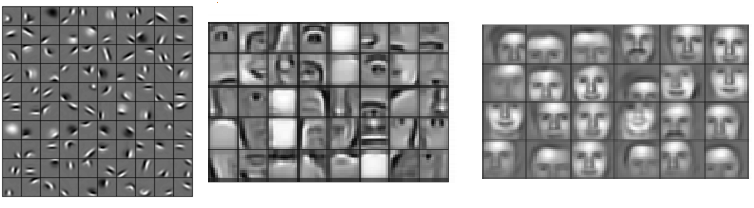
\includegraphics[width=.85\linewidth]{hierarchical_features.png}
 \caption{Learned hierarchical feature learned by Deep Learning algorithm\cite{NvidiaConcepts}}
 \label{fig:FeatLearn}
 \end{center}
 \end{figure}

\section{Logistic Classifier}
The next two sections are going to explain the theory behind deep learning by starting with a logistic classifier and evolving it into a deep network.  The purpose of a logistic classifier is predict a categorical class, given input data.  \textit{Is this an image of a 5? or a 4?}

Throughout all of deep learning the fundamental ingredients are a) Data b) Structure c) Loss and d) Optimizer

\subsection{Data}
As with all supervised machine learning algorithms, it is important to split the data into three sets: training, validation, testing.  Normally, the data is split into 70\% training, 20\% validation, and 10\% testing.  

The training and validation sets are used during training.  The training set is used to adjust the weights of the model.  While the validation set does not update the weights, it is used to validate that the model is not overfitting.  \emph{Overfitting} is when a model is overly complex - it has superfluous freedom to align with the specific data.    

Overfitting can be seen in the following analogy.  A student, analogous to our network model, takes two exams of the same subject repeatedly.  Over many trials the student will improve.  However, if the student's accuracy increases on Test 1 but not on Test 2, then he may be memorizing the answers, not learning the material.  The same is true for our model.  It could be overfitting the training data and not learning the underlying relationship.

The test set is new, unseen data that is only used for testing the final model's predictive power.  To follow the student analogy, the test set is the real world.  

\subsection{Structure}
\subsubsection{Neuron or Node}
The basic building block of a network is the neuron or node (Fig \ref{fig:neuron}).  It takes some input data, applies a linear function to those inputs by calculating a weighted sum, and applies an activation function to that sum.    


\begin{figure}[!h]
 \begin{center}
 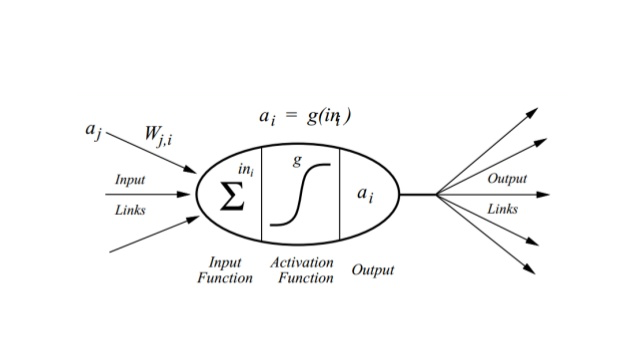
\includegraphics[width=.8\linewidth]{neuron.png}
 \caption{Neuron or node: Basic unit of Deep Learning}
 \label{fig:neuron}
 \end{center}
 \end{figure}
 
 The linear function is defined as 
\begin{equation}
WX+b = Y
\end{equation}
where $X$ denotes an input vector, $W$ denotes a matrix of weights, $b$ denotes the biases, and $Y$ denotes the \emph{scores} or \emph{logits}.  The training happens by trying to find the weights and biases that are good at predicting the correct class.  
For example, take a model that is trying to learn handwritten digits with an input as an image of a handwritten "5."  The linear function (Fig \ref{fig:Lin}) takes that input and outputs logits.  At first these outputs do not mean much.  The task is to determine the probability the image belongs to each class (digit).  The way to turn logits into probabilities is to apply a softmax as our activation function, see Fig \ref{fig:SftMax}.
\begin{figure}[!h]
 \begin{center}
 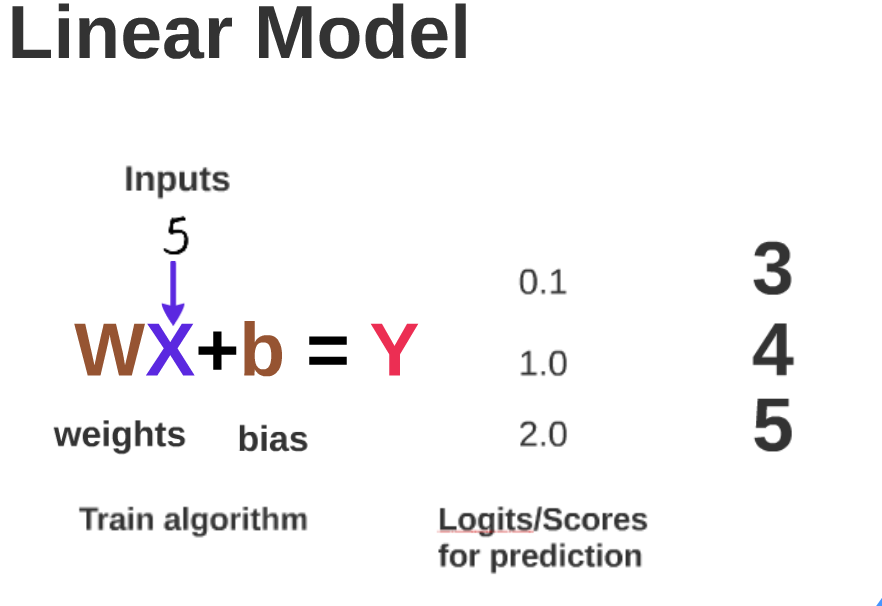
\includegraphics[width=.6\linewidth]{LinFunc.png}
 \caption{Linear Function }
 \label{fig:Lin}
 \end{center}
 \end{figure}
 
\begin{figure}[!h]
 \begin{center}
 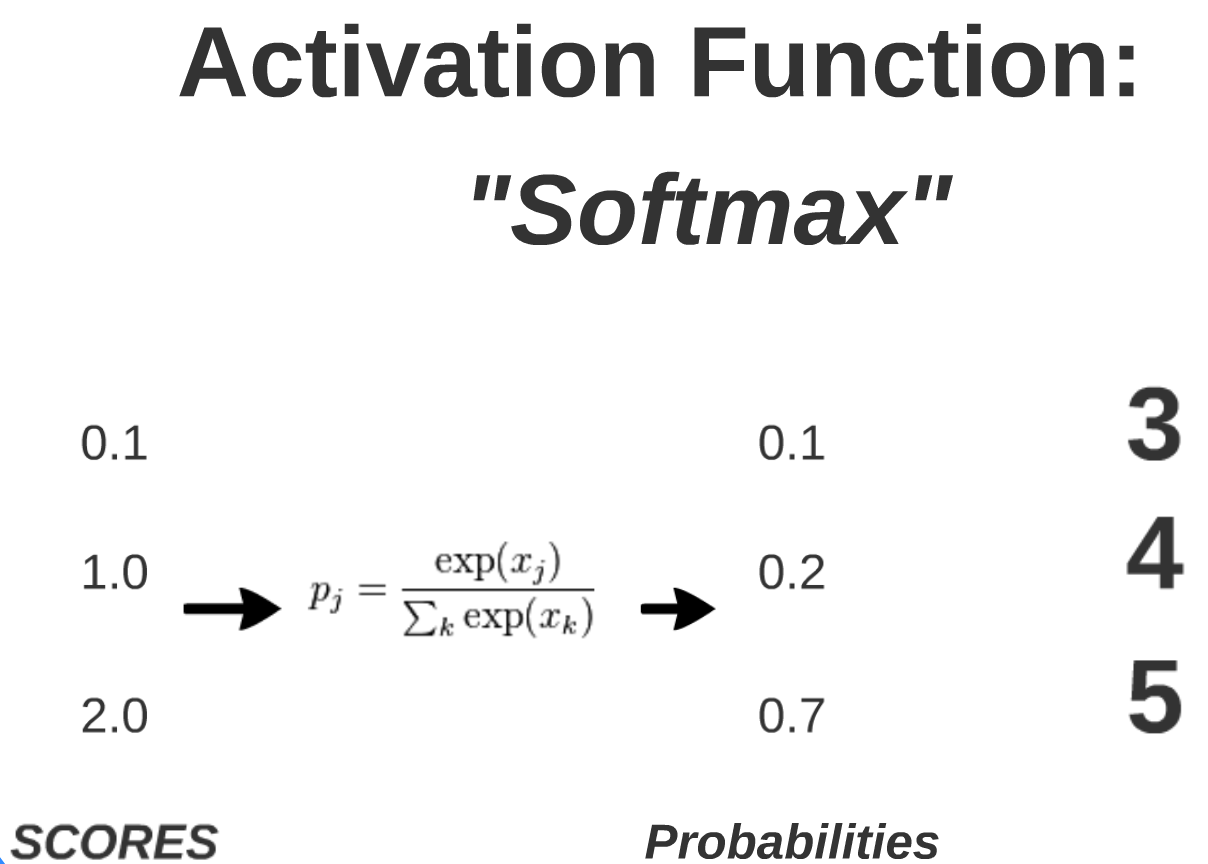
\includegraphics[width=.6\linewidth]{sftMax.png}
 \caption{To turn logits into probabilities, the activation function was chosen to be softmax}
 \label{fig:SftMax}
 \end{center}
 \end{figure}
 
The softmax function outputs the probabilities the image belongs to each class (the most likely is close to 1 and the less likely are close to 0).  The technique of One-hot Encoding is used to turn each label into a class-membership vector.  This vector has the value 1 for the correct class, and 0 for the rest of entries.  In the above example, the five is the correct label, so the one-hot encoded vector is [0,0,1]. 

There are now two vectors, one from the classifier (the probabilities) and one that represents the correct label (encoded vector). 

\subsection{Loss}
For the feedback in the model to work, there must be a metric of success.  The way to measure the distance between potential two vectors is called Cross Entropy, Eq \ref{Eq:X-entropy}. The goal is to have a low distance for a correct class but a high distance for an incorrect one.    
\begin{equation}\label{Eq:X-entropy}
D(S(Y),L)) = \sum_{k}^{ }L_{k}log(S(Y_{k})))
\end{equation}
The Training Loss, Eq \ref{Eq:TrainingLoss}, is defined as the average cross entropy over the entire training set ($i$). A good model has a low training loss.   

\begin{equation}\label{Eq:TrainingLoss}
\mathfrak{L} = \frac{1}{N}\sum_{i}^{ }D(S(WX_{i}+b)),L_{i})
\end{equation}
The loss is a function of the weights and the biases, so we are going to minimize that function using an optimizer.\cite{Udacity} 
\subsection{Optimizer}
One of the most popular optimizing techniques in machine learning is called Stochastic Gradient Descent (SGD).  It takes small steps along the loss surface following the gradient until it finds a minimum.  Recall the gradient is the multivariate slope of a function.  The size of the step is called the \emph{learning rate}.  The bigger the learning rate the faster it learns, but it may not reach the absolute minimal loss.  In practice, SGD is performed over multiple passes of the data set called epochs.  

SGD is popular in machine learning  because it scales well with data and model size.  However, it comes with additional hyper-parameters.  These are different from ordinary parameters that the model optimizes.  Examples of hyper-parameters that the user must tune are:
\begin{itemize}
\item Learning Rate initialization
\item Learning Rate decay
\item Weight initialization
\item Number of Epochs 
\end{itemize}

\subsection{Summary}
To summarize, we have created a linear model that outputs probabilities [structure].  We evaluate how the model is doing by calculating the cross entropy [loss] and use SGD [optimizer] to minimize that loss.  It is still a shallow model, but these are the fundamental tools for going deeper.   
% * <darren@myhigherground.com> 2016-05-19T04:06:28.296Z:
%
% > To summarize, we have created a linear model that outputs probabilities [structure].  We evaluate how the model is doing by calculating the cross entropy [loss] and use SGD [optimizer] to minimize that loss.  It is still a shallow model, but these are the fundamental tools for going deeper.   
%
% awesome paragraph.  give me that same thing in the beginning of the section as part of the intro so i get a better sense of where things are going.
%
% ^.

\section{Deep Learning}
\subsection{MultiLayer Perceptron [MLP]}
To turn the logistic classifier into a network, a second neuron is linked between the current neuron and the input (Fig \ref{fig:basic2L}).  This is called a two-layer Neural Network (the input layer is not counted).   

Layers are the highest level building block of a network.  The new layer is called the Hidden Layer because its output values are not visible to the network output.  The hidden layer gives the model the opportunity to represent the data in a simpler way.

The depth of the network is defined by the number of hidden layers. 

\begin{figure}[!h]
 \begin{center}
 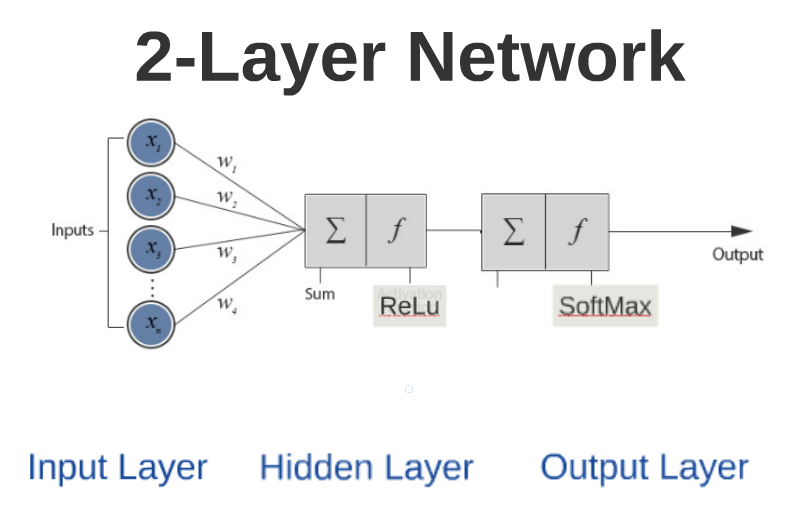
\includegraphics[width=.8\linewidth]{basic_2layer.png}
 \caption{Basic two layer Neural Network}
 \label{fig:basic2L}
 \end{center}
 \end{figure}
In addition to layers, the number of nodes per layer can increase as well.  The number of nodes on a layer represents the degree of freedom of that layer.  

When the output of every node on one layer is connected to the input of every node on the next layer, the network is called \emph{Fully Connected} or \emph{Dense}.  

The size of a network is defined by the number of layers and the number of nodes or parameters.  Fig \ref{fig:NN2} has 2 layers, 4+2=6 nodes (do not count input) or [3x4]+[4x2] = 20 weights and 4+2=6 biases for a total of 26  parameters.  Fig \ref{fig:NN3} has 3 layers, 9 nodes, and 42 learnable parameters.  

Modern convolutional neural networks have 100 million parameters and 20 layers (hence deep learning).  

\begin{figure}[!h]
\centering
\begin{subfigure}{.4\linewidth}
  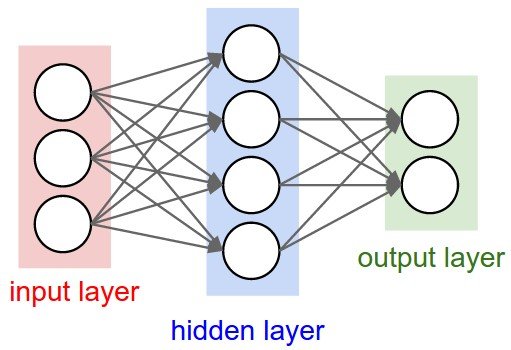
\includegraphics[width=\linewidth]{NN_2layer.jpeg}
  \caption{2-Layer}
  \label{fig:NN2}
\end{subfigure}%
\hfill
\begin{subfigure}{.6\linewidth}
  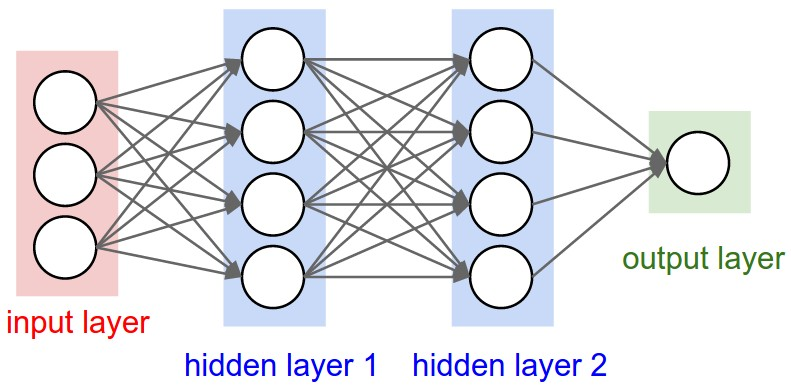
\includegraphics[width=\linewidth]{layerView.jpg}
  \caption{3-Layer}
  \label{fig:NN3}
\end{subfigure}
\caption{Two Fully connected Neural Networks\cite{Stanf}}
\label{fig:test}
\end{figure}

Evolving the structure from a single node into a network has allowed the model more opportunities to represent the data in a simpler way (layers) and more degrees of freedom (nodes).  However, the model is still linear. Because of superposition, stacking a 100 purely linear transformations can be simplified to a single layer. The solution is to introduce non-linear functions.

\subsection{Non-Linearities}
To preserve the network's structure (and the benefits gained with this structure), each hidden layer is given a non-linear activation function.  By adding non-linearity, the entire model is now non-linear and cannot be simplified down to a single transformation.  This creates a hierarchy of abstraction that grows in complexity with every layer.\cite{NvidiaConcepts} \cite{DataWknd}    


This is the foundation for building deep models.    


%Non-linear transformations increase the complexity of the relationships.  In DL, this creates increasingly complex features with every layer.  In contrast, stacking 100 purely linear transformations can be simplified to a single layer.  That is, even when multiple node layers are added, because of superposition, the layers can be rearranged into a single mapping.  For nonlinear layers, the mapping is non-separable - forcing different levels of complexity to be modeled.  
% * <darren@myhigherground.com> 2016-05-19T04:11:23.523Z:
%
% > Non-linear transformations increase the complexity of the relationships.  In DL, this creates increasingly complex features with every layer.  In contrast, stacking 100 purely linear transformations can be simplified to a single layer.\cite{NvidiaConcepts}  That is, even when multiple node layers are added, because of superposition, the layers can be rearranged into a single mapping.  For nonlinear layers, the mapping is non-separable - forcing different levels of complexity to be modeled.  This is the foundation for building deep models. 
%
% you should edit my sentance, but this is a SUPER important paragraph.  i didn't even think about how important this was until you pointed it out.  thats the whole reason its called deep.  neat
%
% ^ <nreis@ucdavis.edu> 2016-05-19T23:04:54.605Z.

There are multiple types of non-linear activation functions: softmax, sigmoidal/logistic, tanh, and the rectified linear unit [ReLU].  A ReLU is a very simple, very powerful non-linearity.  Its output is linear for x greater than zero and zero everywhere else (Fig \ref{fig:ReLU}). Since its introduction in 2012, ReLu has become the most popular non-linearity because it does not face gradient vanishing problems as with sigmoid and tanh function.\cite{DataWknd}


\begin{figure}[!h]
 \begin{center}
 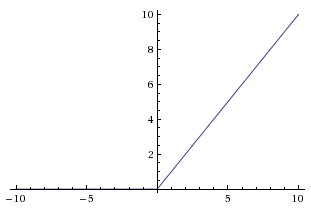
\includegraphics[width=.6\linewidth]{Relu.jpeg}
 \caption{Rectified Linear Unit is the most popular nonlinear function.  }
 \label{fig:ReLU}
 \end{center}
 \end{figure}

\subsection{Summary}
By constructing this MLP network we have given the model a better structure 
\begin{itemize}
\item Hidden Layers - number of moves to figure out a simpler way to represent the data
\item Number of nodes per hidden layer - the degrees of freedom for that move
\item Non-linearities allow increasing feature complexity with each layer  
\end{itemize}
We then told the network to learn the best parameters in order to correctly classify the input.
This is the core to Deep Learning.\cite{Udacity} \cite{DataWknd} \cite{playground}

\section{Convolutional Neural Networks}
Deep networks are powerful but can quickly increase in complexity.  Back to the example of classifying handwritten digits.  If the input image is 32x32 pixels with 3 colors and the network has 2 fully connected layers with 2 outputs (similar to Fig \ref{fig:NN2}) then there would be a total of 9.4 millions learnable parameters.  That is a lot of parameters for a small image and a simple structure.  To help out the model, the user can use his or her domain knowledge (the fact that it is an image).    

Take an image of a cat.  It does not matter where in the image the cat is, it is still an image of a cat.  This is called translational invariance.  Identifying invariant structure is a key aspect in machine learning because it is a direct path to efficient learning.  In a fully connected network, the model learns weights for cats in the right corner and different weights for cats in the left corner.  Instead, the user would like the model to learn features by sharing weights across the entire image.  This is called \emph{convolutions}.   
\subsection{Convolutions}
Fig \ref{fig:CNN} is an example of an input image ($X$)  with a cat in it.  The image has a width, height, and a depth (represented by the RGB colors).  Take a small patch of the image and run a tiny neural network on it with $k$ outputs.  Sliding that patch across the entire image creates a new image with a new width, height, and a depth of $k$.  If the patch was the size of the original image, it would be no different than a fully connected layer.  However, by sweeping a smaller patch across the image  there are fewer weights and the weights are shared across space.  

\begin{figure}[!h]
 \begin{center}
 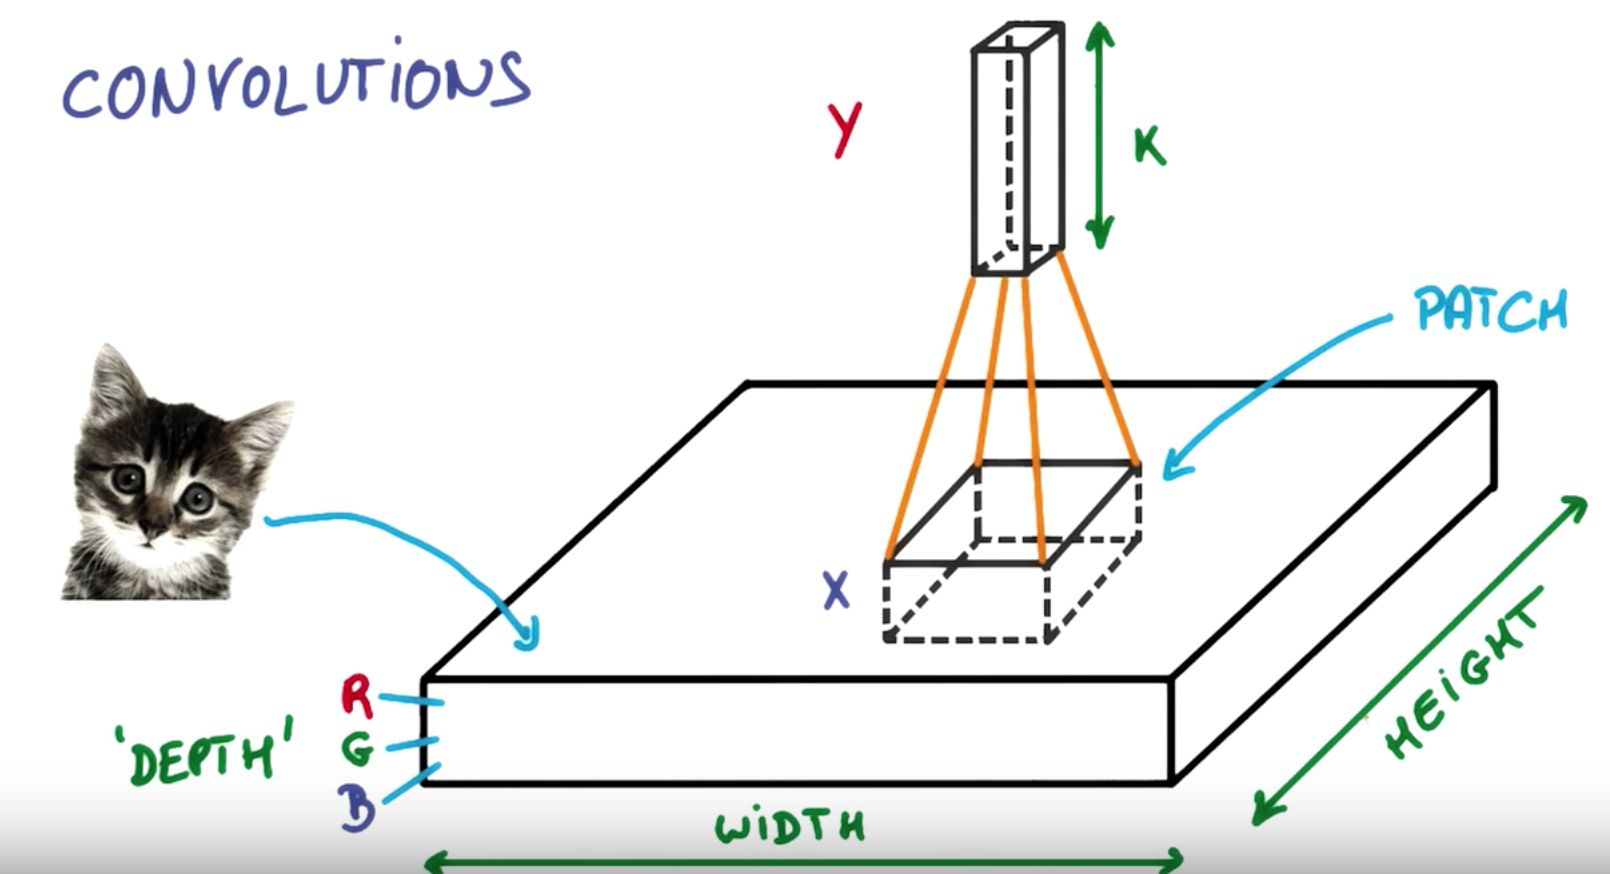
\includegraphics[width=.7\linewidth]{CNN.png}
 \caption{Sketch of how a Convolution passes over an image \cite{Udacity}}
 \label{fig:CNN}
 \end{center}
 \end{figure}

\subsection{Network}
Convolutions are stacked on top of each other to form a convolutional pyramid, Fig \ref{fig:ConvNet}.  The layers progressively squeeze the spatial dimensions, while increasing the network depth.  The depth can be thought of as the semantic representation.  At the end, a fully connected classifier is attached.  Through training, these convolutional layers form the hierarchy of abstraction seen in Fig \ref{fig:FeatLearn}. \cite{Udacity} \cite{DataWknd} 

\begin{figure}[!h]
 \begin{center}
 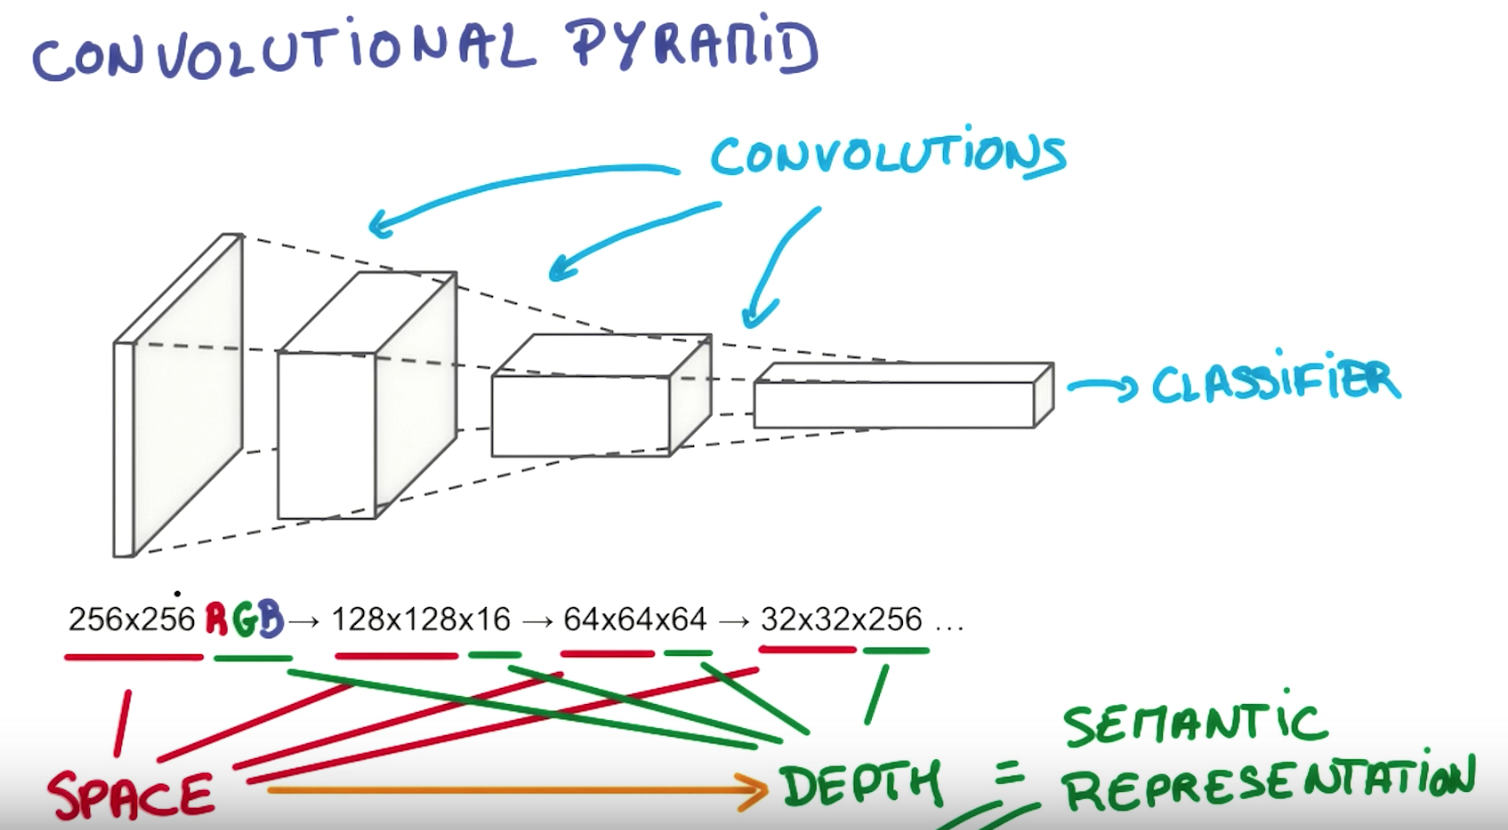
\includegraphics[width=.85\linewidth]{CNN_stack.png}
 \caption{Structure of a ConvNet \cite{Udacity}}
 \label{fig:ConvNet}
 \end{center}
\end{figure}

\section{Example: MNIST}
The challenge of classifying handwritten digits is a classic machine learning problem.  The dataset used is called MNIST and it was one of the first real world problems solved by neural networks.  
\subsection{Data}
MNIST contains 60,000 training images and 10,000 test images of handwritten digits from 500 different writers.  Each image is a grey scale 28x28 pixel image.  10\% of the training data was reserved for validation.  
\subsection{Structure}
Two structures were evaluated: MultiLayer Perceptron [MLP] and a ConvNet.
\subsubsection{MLP}
A 2-Layer Perceptron [MLP] was built with fully connected layers. The input was an image flattened to a vector of length 784 (28x28).  This input was fully connected to a hidden layer with 512 nodes with a ReLU activation function.  The hidden layer was fully connected to the output layer of length 10 (0-9) with a softmax.\footnote{Dropout was applied to combat overfitting}

\subsubsection{ConvNet}
The input image was kept in its original form 1x28x28.  It was inputted into two convolutional layers which squeezed it to a shape of 32x14x14.  That image was fed into the same MLP classifier as described above.
\subsection{Loss and Optimizer}
Both models defined the loss as cross entropy and used RMSprop as their optimizer.  [RMSprop is a version of SGD with an adaptive learning rate].
\subsection{Results}
The results are shown in the Table \ref{tbl:MNIST} below.  Both algorithms performed excellent. Out of the 10,000 test points, the MLP missed 188.  The  ConvNet misclassified only 93;  it was twice as accurate in half the number of epochs.  Fig \ref{fig:MNIST} shows the loss curves for each, demonstrating that neither model overfit the training data.  The time per epoch was listed because this example was done on the author's personal computer (2014 13in Macbook Pro running OS X 10.11.4, 2.6GHz 8GB, Intel Iris 1536MB).  At the time of purchase, the author had no intention of demanding more than basic performance from his machine.  Had this experiment been run on a GPU the training time would have been an order of magnitude faster.  


\begin{table}[h!]
\centering
\caption{Results from Classifying MNIST}
\label{tbl:MNIST}
\resizebox{\linewidth}{.3in}{%
\begin{tabular}{ccc|ccc}
\hline
\multicolumn{1}{l}{} & \multicolumn{1}{l}{} & \multicolumn{1}{l|}{} & \multicolumn{3}{c}{Accuracy}            \\ \hline
                     & Epochs               & time per Epoch [s]    & Training Set & Validation Set & Test Set \\ \cline{2-6} 
MLP                  & 10                   & 10                    & 0.9822       & 0.9828         & 0.9812   \\
CNN                  & 5                    & 360                   & 0.9928       & 0.9915         & 0.9907   \\ \hline
\end{tabular}%
}
\end{table}


\begin{figure}[!h]
\centering
\begin{subfigure}{.5\linewidth}
  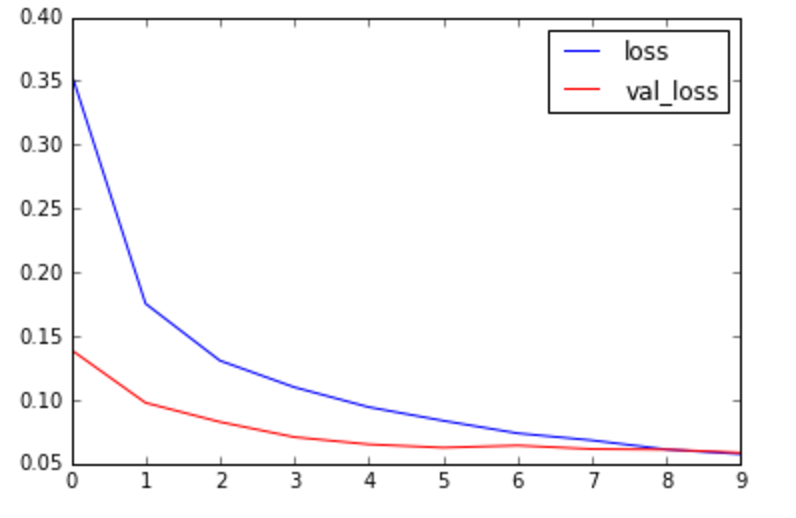
\includegraphics[width=\linewidth]{MLP.png}
  \caption{MLP}
  \label{fig:MLP}
\end{subfigure}%
\hfill
\begin{subfigure}{.5\linewidth}
  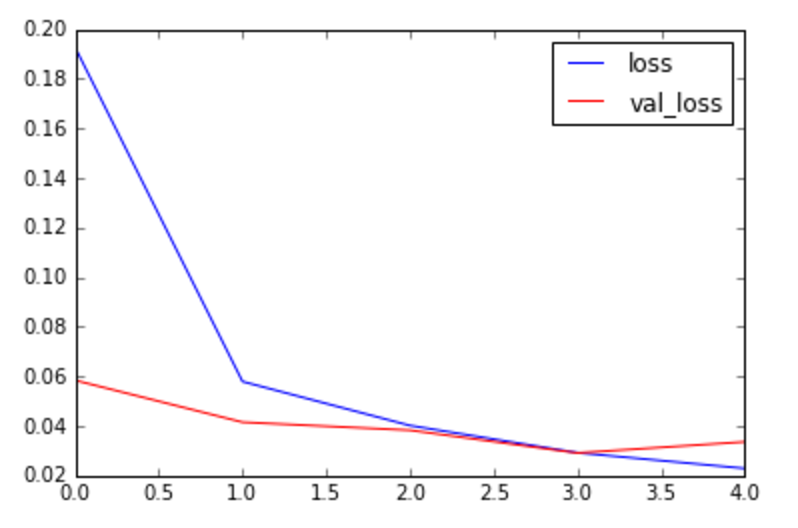
\includegraphics[width=\linewidth]{CNN_loss.png}
  \caption{ConvNet}
  \label{fig:NN3}
\end{subfigure}
\caption{Loss as a function of epoch.  The fact that the training and validation losses converge is evidence that the model is not overfitting}
\label{fig:MNIST}
\end{figure}

\section{Tools}
The good news is that the field of DL is exploding and a majority of it is open-source.  The bad news is that this field is in its infancy so there are a lot of options and it is difficult to configure your system.  
 
\subsection{Programming}
Deep learning is programmed in mostly Python or C++. Since it is just math, one can program all of the operations from scratch.  However, many common functions have been built into open-source toolkits.  The community has not consolidated yet, so there are over 50 different toolkits, each with its advantages and disadvantages.  The most popular include
\begin{itemize}
\item TensorFlow
\item Keras
\item Theano
\item Caffe
\item Torch
\item CNTK
\end{itemize}

Google open-sourced its toolkit called TensorFlow and it has gained a lot of traction in the six months since its release (November, 2015).  It is a very powerful toolkit that they are writing all of their algorithms on.  

The best place to start is a toolkit called Keras.  It is built to run on top of TensorFlow or Theano.  The purpose of this toolkit is to enable fast, easy prototyping.  While it is not as powerful as other options it allows beginners to get their hands dirty quickly. \footnote{It is this author's opinion that creating an environment inside anaconda was the most successful way to get started.}

In addition to toolkits, existing pre-trained networks are usually open-sourced.  Winning networks, such as AlexNet (the first ConvNet submitted to ImageNet), open-source their learned parameters and structure.  

\subsection{Transfer Learning}
One of the continuing limitations of DL is data.  While the amount of data is increasing exponentially, getting good, clean data is hard to come by.  Large corporations like Facebook or Google can pay for manual labeling of data, but everyone else uses shared data sets like MNIST over and over again.  Few DL models are trained from scratch.  It is logical to assume that is would stall innovation; however, this is not true.  It has been shown that CovNets learned from large data sets can learn generic features and be repurposed for other smaller databases. \cite{lin2015learning} 

\begin{figure}[!h]
 \begin{center}
 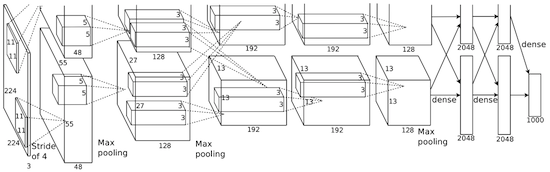
\includegraphics[width=.8\linewidth]{alexnet_small.png}
 \caption{The structure of AlexNet  \cite{AlexNet}}
 \label{fig:AlexNet}
 \end{center}
\end{figure}

\subsubsection{Fine Tuning}
Take a ConvNet pre-trained on ImageNet and cut off the last fully connected layer (that classifies the 1000 classes defined by ImageNet).  Retrain the CovNet by fine-tuning the existing weights for this new dataset. Essentially, the original weights are used as an initialization for the new task.  The motivation behind this strategy is that the lowest levels of the ConvNet contain generic features (edge detector or blob) that can be useful for many task; however, later layers become progressively more specific to the nuances of the classes for the original dataset.   For example, ImageNet has a number of dog breeds, so AlexNet likely has a number of later filters that can distinguish between the breeds. \cite{Stanf} 


\subsection{Technology}
As previously stated, the exponential rise in computational power has enabled DL to grow at an incredible rate.  In the 2000s, researchers recognized that the GPU inside gaming computers was perfect for quickly multiplying very large matrices.  They originally rode the rise of gaming computers, but lately, computer companies, like Nvidia, have taken notice of DL and begun building chips specifically designed for DL.  Deciding which GPU specifications is beyond the scope of this report but there are many resources for those who are interested. \cite{GPUs}  

Another option is Amazon Web Services [AWS].  A user can rent time on Amazon's GPUs to run an algorithm for a couple hours.  This is great for testing models out without the investment in hardware.  




\cleardoublepage

\chapter{U-Net architecture}
\label{ch:u_net_architecture}

In the few years, deep convolutional networks have outperformed the state of the art in many visual recognition tasks. While convolutional networks have already existed for a long time their success was limited due to the size of the available training sets and the size of the considered networks.

The typical use of convolutional networks is on classification tasks, where the output to an image is a single class label. However, in many visual tasks, especially in biomedical image processing, the desired output should include localization, i.e., a class label is supposed to be assigned to each pixel. Moreover, thousands of training images are usually beyond reach in biomedical tasks. Hence trained a network in a sliding-window setup to predict the class label of each pixel by providing a local region (patch) around that pixel as input. First, this network can localize. Secondly, the training data in terms of patches is much larger than the number of training images.

U-net was originally invented and first used for biomedical image segmentation. Its architecture can be broadly thought of as an encoder network followed by a decoder network. Unlike classification where the end result of the the deep network is the only important thing, semantic segmentation not only requires discrimination at pixel level but also a mechanism to project the discriminative features learnt at different stages of the encoder onto the pixel space. 


The encoder is the first half in the architecture diagram \ref{fig:unet}. It usually is a pre-trained classification network like VGG/ResNet where you apply convolution blocks followed by a maxpool downsampling to encode the input image into feature representations at multiple different levels.

The decoder is the second half of the architecture. The goal is to semantically project the discriminative features (lower resolution) learnt by the encoder onto the pixel space (higher resolution) to get a dense classification. The decoder consists of upsampling and concatenation followed by regular convolution operations.

\begin{figure}[!h]
\begin{center}
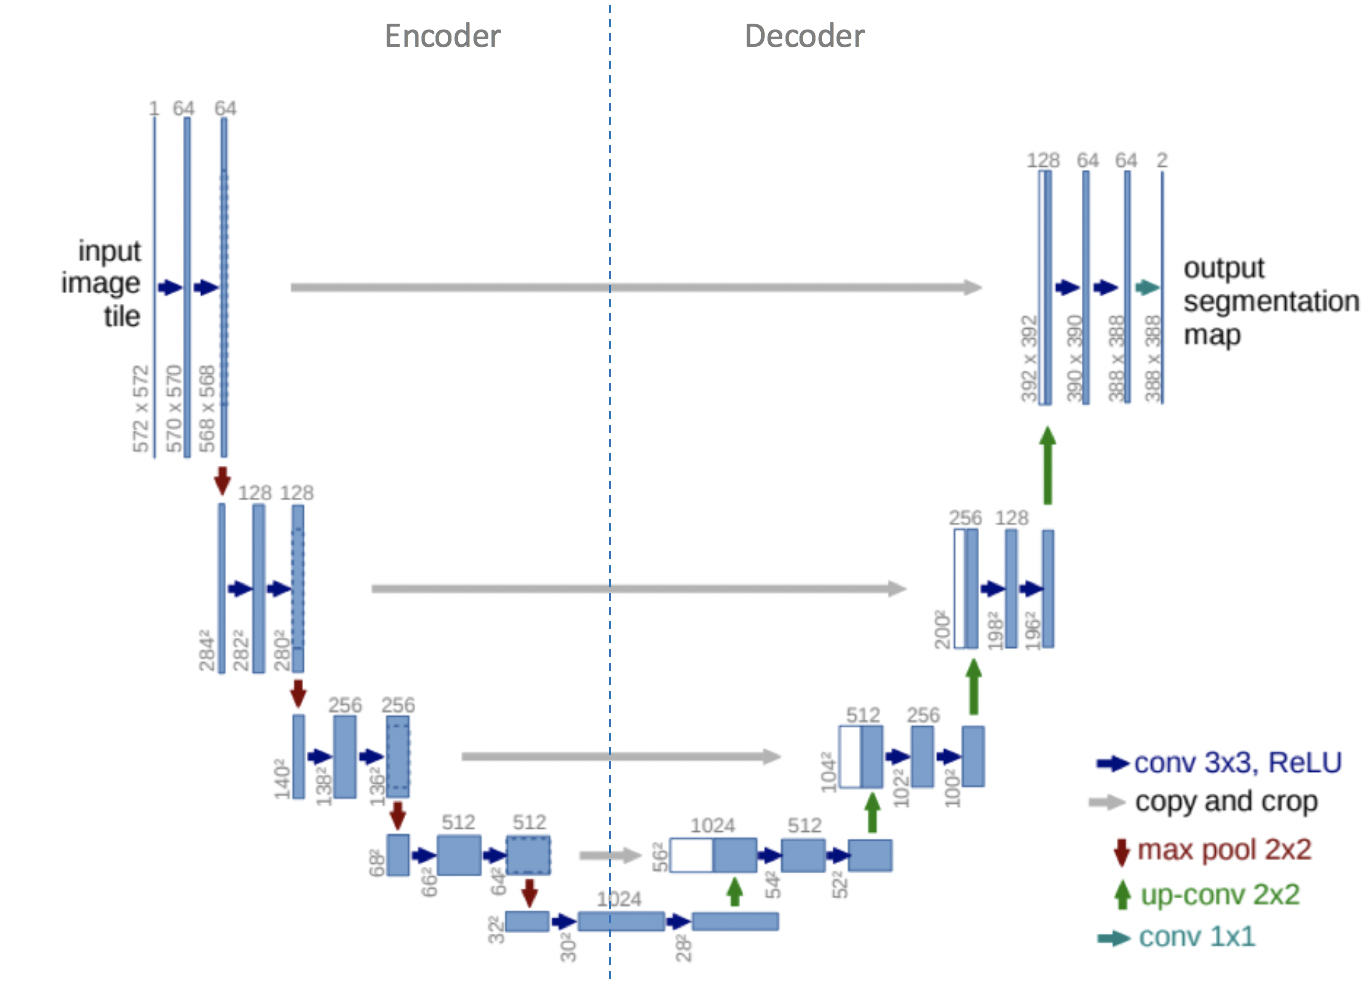
\includegraphics[width=.7\linewidth]{images/unet.png}
\caption {U-net architecture. Blue boxes represent multi-channel feature maps, while while boxes represent copied feature maps. The arrows of different colors represent different operations.} 
\label{fig:unet}
\end{center}
\end{figure}

The intuition is that we would like to restore the condensed feature map to the original size of the input image, therefore we expand the feature dimensions. Upsampling is also referred to as transposed convolution, upconvolution, or deconvolution. There are a few ways of upsampling such as Nearest Neighbor, Bilinear Interpolation, and Transposed Convolution from simplest to more complex.

In summary, unlike classification where the end result of the very deep network is the only important thing, semantic segmentation not only requires discrimination at pixel level but also a mechanism to project the discriminative features learnt at different stages of the encoder onto the pixel space.
\cleardoublepage

\chapter{Methods}
\label{ch:methods}

It was used two CNNs, first a detection model which segments the vertebrae from the background (see Figure 5.1 1a.), then an identification model which identifies which pixels belong to which vertebra (see Figure 5.1 1c). 

\begin{figure}[!h]
\begin{center}
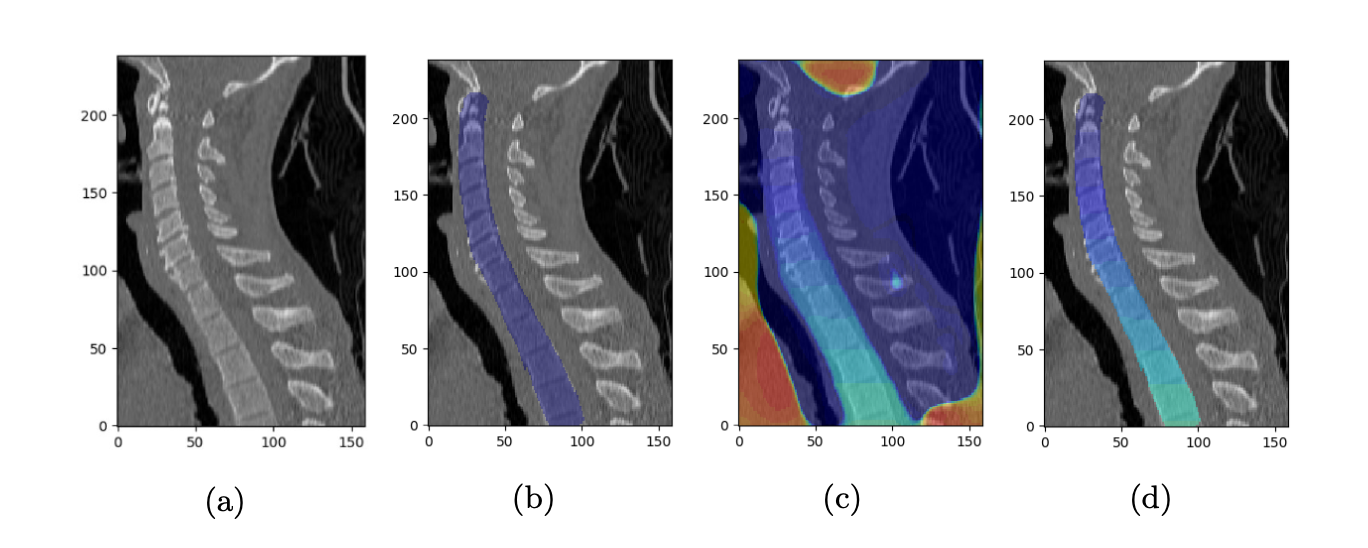
\includegraphics[width=.7\linewidth]{images/verteb_det_loc.png}
\caption {(a) shows an original scan in grey scale, (b) shows the output of the detection model applied to the scan, (c) shows the output of the identification model applied to the scan, (d) shows (b) and (c) multiplied together to produce a final prediction for each pixel.} 
\label{fig:verteb_det_loc}
\end{center}
\end{figure}

This approach was arrived at by analyzing how we could capture the ordering of the vertebrae. The identification model does not classify each pixel discretely but instead produces a continuous value for each pixel. This value is then rounded to an integer which corresponds to a specific vertebra, for example 4 = C4 vertebra. This means we can use an L1 loss function on each pixel and thus capture the ordering through this loss function. This approach would not have been possible if we had included background pixels in the identification stage therefore we segment out the background in the detection step. Our approach also captures short-range and long-range information, 3D short-range information is captured in the detection model by feeding in small 3D samples to train the network. The identification model is trained by feeding in large slices which capture long-range information, which is essential for the task of identifying individual vertebrae. To produce our final dense predictions we multiply the results of the detection model and identification model to produce a labelling on each pixel (see Figure 5.1 1d). These final predictions are then aggregated to produce final centroid estimates for each vertebra.


\subsection{Detection Model}
The detection model classifies each pixel of a scan as either ‘background’ or ‘vertebrae’1. To train the network we feed in 5 cropped samples for each scan in the training set (enforcing that at least 4 of them contain some vertebrae pixels), each sample has size 64 x 64 x 80 pixels. 

Each sample has an accompanying dense labelling, containing 0s (for background) and 1s (for vertebrae), of the same size, for the network to learn from. A 3D U-net architecture was used as portrayed in \ref{fig:detection_model_architecture}). We used a weighted categorical cross entropy loss with 2 classes as our loss function. We gave the background label a 0.1 weighting and the vertebrae label a 0.9 weighting to reflect the proportion of background labels in the samples. 
The full loss function is shown in Eq.(\ref{loss_function}) 
\begin{equation}\label{loss_function}
L(P,Q) = 0.1 * P(\theta) * \log_Q(\theta) + 0.9 * P(1)\log_Q
\end{equation}

\begin{figure}[!h]
\begin{center}
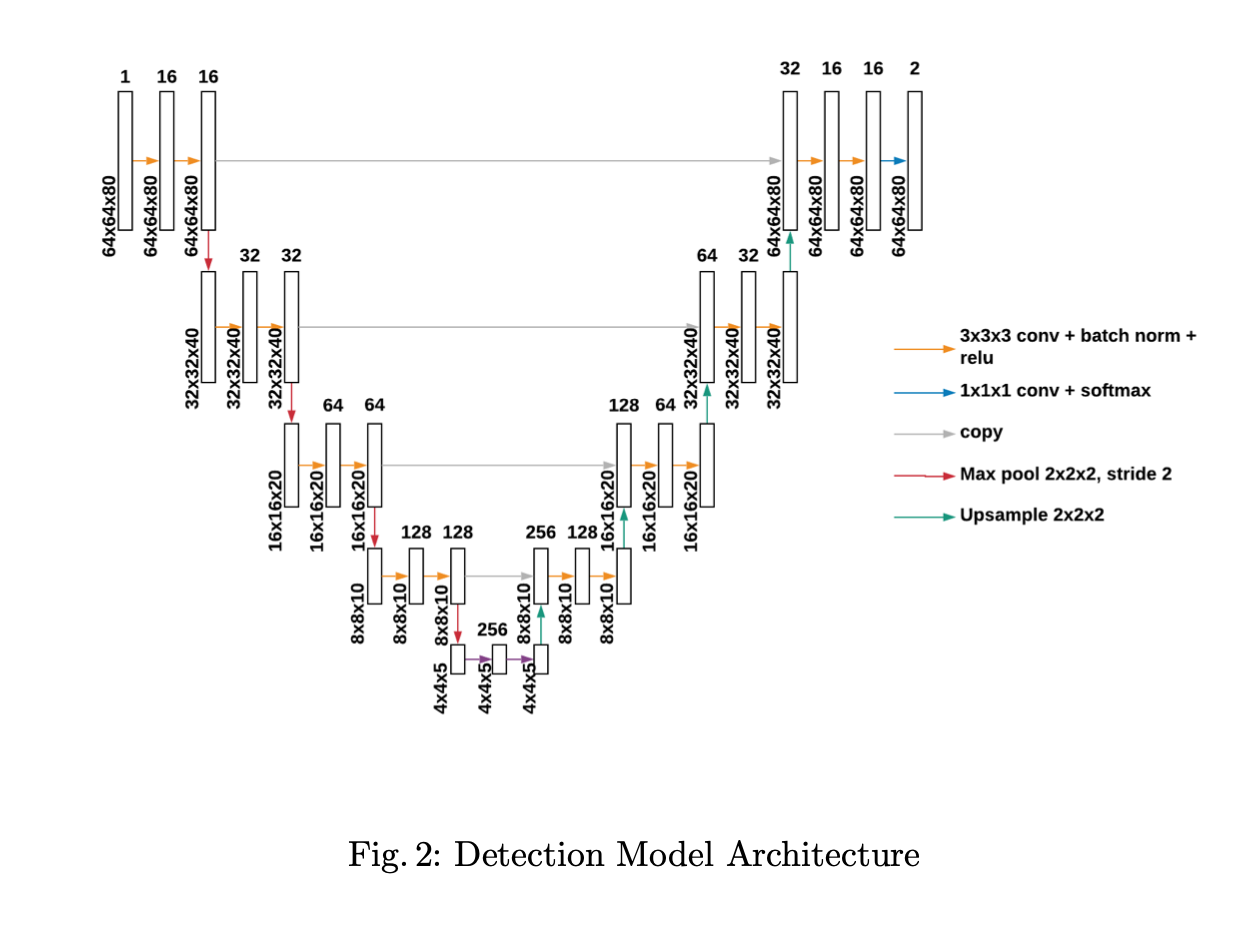
\includegraphics[width=.5\linewidth]{images/detection_model_architecture.png}
\caption {Detection Model Architecture} 
\label{fig:detection_model_architecture}
\end{center}
\end{figure}

It was used ’same’ padding for all convolutional layers with stride $1$, a learning rate $\lambda$ of $0.001$, a batch size of $16$, batch normalization after every convolutional layer with momentum of $0.1$ and trained for $50$ epochs which took $> 11$ hours on the hardware. There was obtained a validation Dice score of $0.961$ on the 1 (vertebrae) labels and a validation accuracy of 98.5\% on test samples generated from our test set.

At test time the applied detection model which scan patch-wise with some overlap between patches. The input to the network is $64 x 64 x 80$ and in steps of $32 x 32 x 40$, padding the border of the scan by $16 x 16 x 20$ and discarding the outer border of size $16 x 16 x 20$ from each output. This reduced edge artifacts in the detection and led to improved mean localization scores.

\subsection{Identification Model}
The identification model outputs a continuous value for each pixel of a scan which, is rounded to an integer to correspond to a specific vertebrae. The identification model gives a value to each pixel even if that pixel is not depicting any vertebrae and is a background. These pixels will be filtered out of the final predictions by multiplying them by their corresponding pixel from the output of the detection model which should be $0$ for a background pixel. To train the identification network it was feed in cropped samples of size $8 x 80 x 320$, generate $100$ cropped samples for each scan in the training set (enforcing that all of them capture some vertebrae pixels), each with a corresponding dense labelling of size $80 x 320$, representing the labelling for the fourth slice of the input sample. Also elastically deform each of these samples along the 2nd and 3rd axis using the elastic-deform python package. (with $\sigma$ = 0.7 on $\alpha$ $3 × 3$ grid).

It was established 2D U-net architecture for the identification model with $8$ channels in the input layer to pass in our samples of size $8 x 80 x 320$. Implemented U-net architecture with large anisotropic filters of size $5 x 20$ at the lowest level of the architecture to increase the size of the receptive field thus maximizing the contextual information captured by the network (\ref{fig:identification_model_architecture}). 

\begin{figure}[!h]
\begin{center}
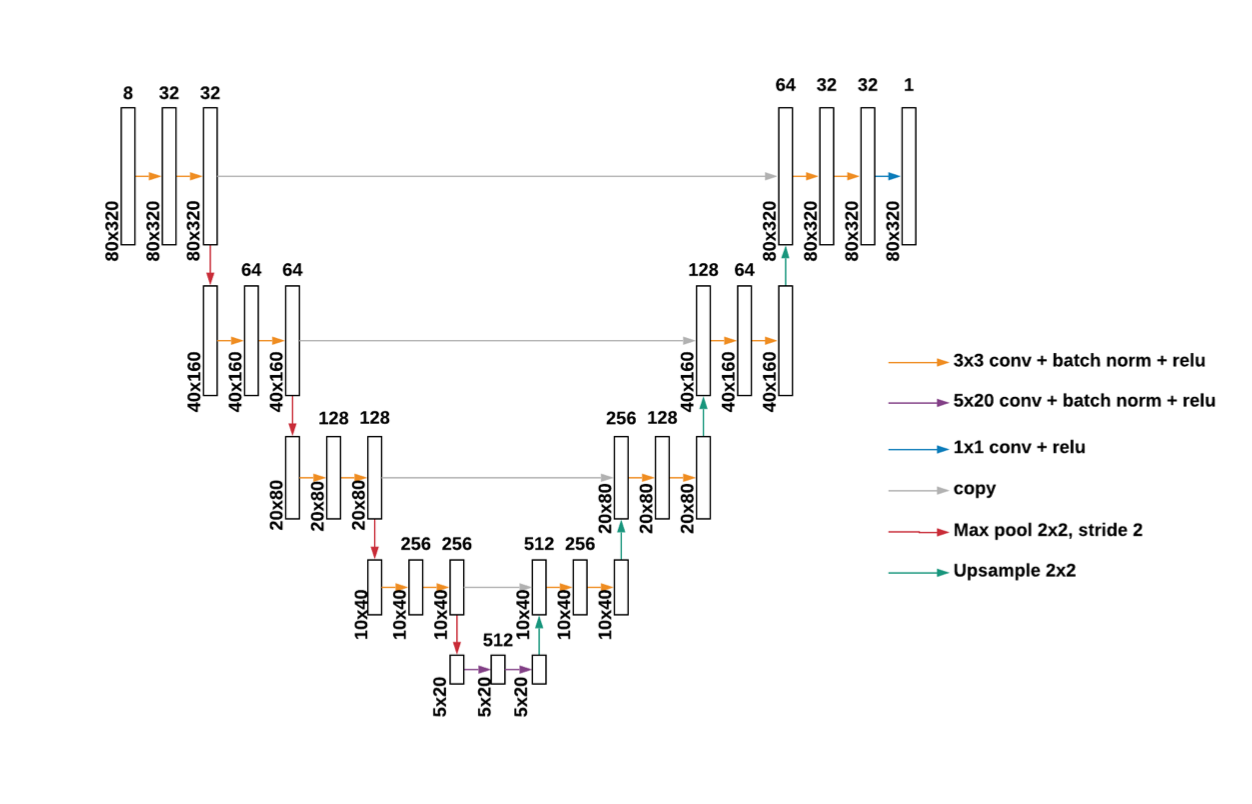
\includegraphics[width=.5\linewidth]{images/identification_model_architecture.png}
\caption {Identification Model Architecture} 
\label{fig:identification_model_architecture}
\end{center}
\end{figure}

As mentioned previously, pixels which are background will be filtered out by multiplying by the detection model. This means that we do not care about the pixels which are labelled as background when we train this model. This is reflected in the loss function which is a modified L1 loss function given below (\ref{l1_loss}):

\begin{equation}\label{l1_loss}
L = \begin{cases} \lvert $y_i$ - $x_i$ \rvert, & \mbox{if } \mbox{$x_i = 0$} \\ 
    0, & \mbox{otherwise } \end{cases}
\end{equation}
Where $y_i$ is the predicted value of pixel $i$ and $x_i$ is the true value of pixel $i$.

It was used ’same’ padding for all convolutional layers with stride $1$, a learning rate $\lambda$ of $0.001$, a batch size of $32$, batch normalization after every convolutional layer with momentum of $0.1$ and trained for $35$ epochs which took $> 7$ hours.
The identification model is a fully convolutional network which allows us to apply it to whole slices of the input scan, padded to the nearest multiple of $16$, at test time.

\subsection{Sparse to Dense Annotation}
To train both the detection and the identification model we feed in samples each with a corresponding dense labelling. In the case of the detection model the dense labelling contains two values; 0 representing background and 1 representing vertebrae (see \ref{fig:annotated_scan} b). The identification model’s dense labelling contains values from 0 to 26, 0 representing background, 1 representing C1 vertebrae etc... up to 26 representing S2 vertebrae (see \ref{fig:annotated_scan} c). Dataset comes with centroid positions (sparse labels) which must be converted to dense labels. This approach however is not the most accurate dense labelling because vertebrae are not spherical. Implemented algorithm which produces an anatomically better dense labelling, which is a better approximation of which pixels are vertebrae (detection) and which vertebra those pixels correspond to (identification), from the ground-truth sparse annotations.

The algorithm steps can be represented as:
\begin{itemize}
    \item Find midpoints between all adjacent centroids in the column.
    \item Draw line segments between these midpoints. Add additional line segments at the start and end of the column so that there is a line segment to represent
each vertebra.
    \item  Plot discs (on the plane of the sagittal and transverse axes) around each point on the line segment. The radius of these discs is specific to the vertebra the line segment represents. 
    \item Result: approximations of the radii for specific vertebrae.
\end{itemize}

\begin{figure}[!h]
\begin{center}
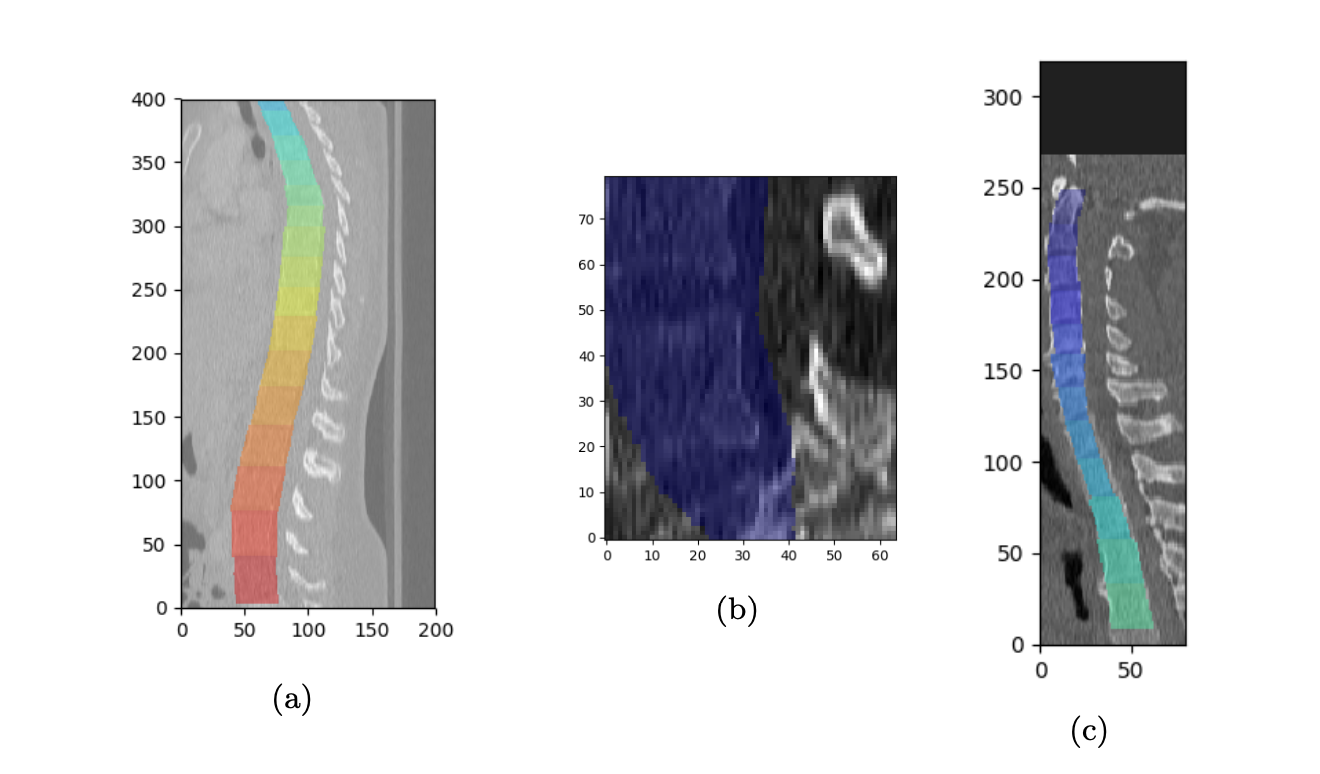
\includegraphics[width=.5\linewidth]{images/annotated_scan.png}
\caption {(a) shows a dense labelling, (b) shows an example of a sample used to train the detection model (the sample is 64 x 64 x 80 but only a 64 x 80 slice is shown here). Note: any value over 1 in the dense labelling is converted to 1 for the detection model samples, (c) shows an example of a sample used to train the identification model. Note: The size of the sample is 8 x 80 x 320, if the original scan is not larger enough to fill those dimensions some padding is added, as can be seen at the top.} 
\label{fig:annotated_scan}
\end{center}
\end{figure}


\subsection{Dense to Sparse Annotation}
Once a label has been predicted for each pixel (see \ref{fig:verteb_det_loc} d) these labels are aggregated to calculate predicted centroid positions. To aggregate we find the median position of all pixels which vote for each vertebra. However before calculating this we apply a threshold so that if there are less than a certain number of pixels voting for a vertebra we do not include that centroid in the prediction. This filters out erroneous predictions produced by the identification model.
The threshold $x_v$ is specific to the vertebra $v$ and is calculated using Eq.\ref{x_v threshold}

\begin{equation}\label{x_v threshold}
x_v = max(3000, 0.4R_v^3)
\end{equation}
where $R$ is the radius of the vertebra $v$. 
\cleardoublepage

\chapter{Experiments}
\label{ch:experiments}


\section{Machine properties}
Within the experiments it was used macbook pro middle 2018 with Coffee Lake/8th generation: a 2.2GHz Core i7 processor with six cores and with intel turbo boost up to 4.1GHz.

\section{Data}
The experimental \ref{fig:ct_spine} data set was splitted into dedicated training (with ground-truth labels) and test sets each 242 and 60 scans accordingly. The scans were re-sample  at 1mm x 1mm x 1mm resolution meaning each pixel in the generated samples from the scans provided a 3 dimensional 1mm section of the patient spine.
\begin{figure}[h]
    \centering 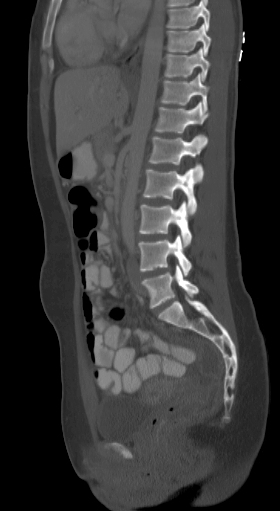
\includegraphics[width=3cm]{images/ct-spine.jpg}
    \caption {Train sample of CT spine scan}
    \label{fig:ct_spine}
\end{figure}


\section{Training detection model}
trained for 50 epochs which took 11 hours. obtained a validation Dice score of 0.961 on the 1 (vertebrae) labels and a validation accuracy of 98.5 on test samples generated from test set.
At test time applied the detection model to a scan patch-wise with some overlap between patches. The input to the network is 64 x 64 x 80 and we applied it in steps of 32 x 32 x 40, padding the border of the scan by 16 x 16 x 20 and discarding the outer border of size 16 x 16 x 20 from each output. This reduced edge artifacts in the detection and led to improved mean localization scores.

\section{Training identification model}
trained for 35 epochs which took 7 hours.
The identification model is a fully convolutional network which allows us to apply it to whole slices of the input scan, padded to the nearest multiple of 16, at test time.


\section{Results}
results are calculated over the dedicated testing set of
60 scans. measured metrics, Id rate, mean localization distance and standard deviation (std) distance. Id rate is the percentage of the centroid estimations predicted which are closest to the correct ground truth vertebra centroid (and are less than 20mm from that centroid). Mean and Std relate to the localization error distance between the predicted centroid positions and the ground-truth centroid positions for the same vertebrae (if it occurs in the scan).

%
- competitors

%
- table of comparison
\cleardoublepage

\chapter{Results}
\label{ch:results}

The results reported are calculated over the dedicated testing set of $60$ scans. It was measured metrics, $Id rate$, $mean localization distance$ and $standard deviation (std) distance$. $Id rate$ is the percentage of the centroid estimations predicted which are closest to the correct ground truth vertebra centroid (and are less than $20mm$ from that centroid). $Mean$ and $Std$ relate to the localization error distance between the predicted centroid positions and the ground-truth centroid positions for the same vertebrae (if it occurs at the scan). 

Table \ref{results_table} represents a performance of the method.
It performs slightly worse on the Id rate. A possible reason for this is that our method relies on the ordering of vertebrae and sufficient contextual information to localize in a dense regression identification stage, but it does not explicitly classify vertebrae, for example, using categorical cross entropy. 

\begin{figure}[!h]
\begin{center}
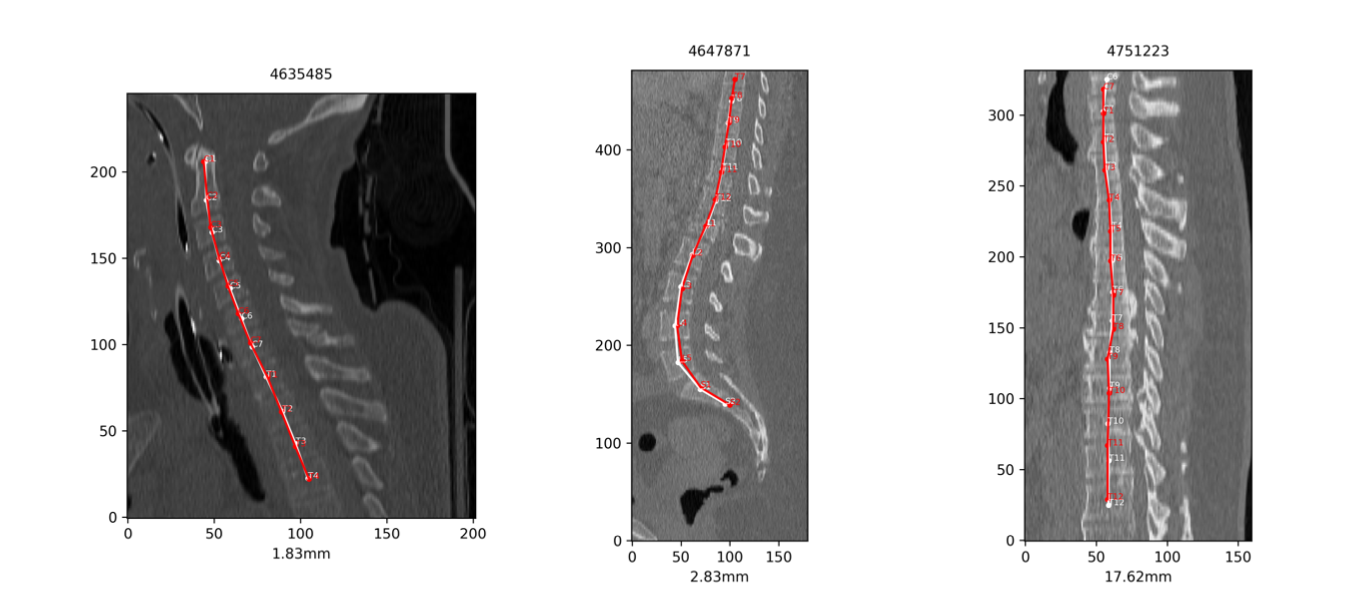
\includegraphics[width=.5\linewidth]{images/3_predictions.png}
\caption {Example of 3 predictions, the red points are method’s centroid predictions, the white points are the ground-truth centroid locations, below each scan the mean localization error for that scan is shown as well.} 
\label{fig:3_predictions}
\end{center}
\end{figure}

The advantage of the method is that it is lightweight and fast both in training time, models took $> 11 hours$ (detection model) and $> 7 hours$ (identification model) to train, but also at test time, with predictions for a scan being computed on average in $40 seconds$. The method does not rely on an iterative stage and usage of RNN, thus making the method likely more efficient at test time.

\begin{center}\label{results_table}
\begin{tabular}{ c c c }
 ID rate & Mean & Std \\ 
 85.8\% & 5.60 & 7.10 \\  
 90.6\% & 3.93 & 5.27 \\
 79.8\% & 6.61 & 7.40 \\
 92.0\% & 5.39 & 8.70 \\
\end{tabular}
\end{center}



\cleardoublepage

\chapter{Conclusion}
\label{ch:conclusion}
Accordingly  accomplished and presented job within the thesis work we may enclose CNNs effectively cope with extracting the features of vertebral samples by leveraging the domain information contained in certain vertebrae scans.

The two stage CNN pipeline which initially detect vertebrae then identify specific vertebrae keening with a 2-class cross entropy loss  and L1 loss accordingly outcomes spectacular results for vertebrae segmentation problem on a publicly available pathological spine CT data set. The full project codebase within the step-wise instructions is hosted at the author's github repository \footnote{ \url{https://github.com/KumundzhievMaxim/VertebraeSegmentation}}
\cleardoublepage

% Irodalomjegyzék (kötelező)
% Bibliography (mandatory)
\addcontentsline{toc}{chapter}{\biblabel}
\printbibliography[title=\biblabel]
\cleardoublepage

% Ábrajegyzék (opcionális) - 3-5 ábra fölött érdemes
% List of figures (optional) - useful over 3-5 figures
%\addcontentsline{toc}{chapter}{\lstfigurelabel}
%\listoffigures
%\cleardoublepage

% Táblázatjegyzék (opcionális) - 3-5 táblázat fölött érdemes
% List of tables (optional) - useful over 3-5 tables
%\addcontentsline{toc}{chapter}{\lsttablelabel}
%\listoftables
%\cleardoublepage

% Forráskódjegyzék (opcionális) - 3-5 kódpélda fölött érdemes
% List of codes (optional) - useful over 3-5 code samples
%\addcontentsline{toc}{chapter}{\lstcodelabel}
%\lstlistoflistings
%\cleardoublepage

% Jelölésjegyzék (opcionális)
% List of symbols (optional)
%\printnomenclature

\end{document}
